\documentclass[12pt]{article}
\usepackage{graphicx} % Required for inserting images
\usepackage[top=1.7cm,bottom=1.7cm,left=2cm,right=2cm]{geometry}
\usepackage[french]{babel}
\usepackage{amsmath}
\usepackage[utf8]{inputenc}
\usepackage[T1]{fontenc}
\usepackage{ulem}
%\usepackage{minted}
\usepackage{listings}
\usepackage{caption}
\usepackage{subcaption}
\usepackage{ragged2e}
\usepackage{amsmath}
\usepackage{xcolor} % to access the named colour LightGray
\definecolor{LightGray}{gray}{0.9}
\usepackage{pifont}
\usepackage[hidelinks]{hyperref}
\usepackage{wrapfig}
%\usepackage{floatrow
\usepackage{changepage}
\usepackage{multicol}
%\usepackage{setspace}
%\onehalfspacing
%\usepackage{mathptmx} %times new roman
\newcommand{\unit}[1]{\ensuremath{\, \mathrm{#1}}}









% Page de garde
\begin{document}
\begin{titlepage}
    \centering
    
    % Logo de l'Institut
    
\includegraphics[width=0.4\textwidth]{Logo/logo_institut.jpeg} 
\includegraphics[width=0.4\textwidth]{Logo/UPSaclay.jpg}

    % Titre du sujet
    \vspace{2cm}
    {\LARGE\textbf{Rapport de stage}\par}
    
    % Informations sur l'étudiant
    \vspace{2cm}
    {\large\textbf{Arnaud COSTERMANS et Achile PINSARD}\par}
    
    % Année universitaire
    \vspace{0.5cm}
    Année universitaire : 2022-2023
    
    % Année d'études et nom de l'Institut
    \vspace{0.5cm}
    Année d'études : Promotion 2024 (L2) \\
    Licence de Science et Technologie \\
    Institut Villebon - \textit{Georges Charpak}
    
    % Informations sur le laboratoire/entreprise
    %\vspace{2cm}
    %\includegraphics[width=0.2\textwidth]{logo_laboratoire}
    
    % Nom et adresse du laboratoire/entreprise
    %\vspace{0.5cm}
    %\textbf{Nom du Laboratoire/Entreprise}\\
    %Adresse du Laboratoire/Entreprise
    % Nom du maître de stage
    \vspace{0.5cm}
    Maître de stage : Cyril DAUPHIN
    
    % Nom de l'enseignant référent
    \vspace{0.5cm}
    Enseignante référente : Martine THOMAS
    
    % Durée du stage ou date de soutenance
    \vspace{0.5cm}
    Stage effectué du 15/05 au 13/06 
\end{titlepage}
\newpage
\begin{adjustwidth}{30pt}{30pt}
%\maketitle

\begin{center}
    \subsubsection*{Remerciement}

Nous aimerions remercier Cyril DAUPHIN ainsi que l’Institut Villebon - \textit{George Charpak} de nous avoir accueillis pour ce stage. 
\end{center}
\begin{center}
    \subsubsection*{Résumé}
\end{center}
Ce rapport de stage présente le travail que nous avons effectué sur l’étude de transfert radiatif d’un modèle à deux faisceaux lumineux.
Actuellement, le modèle à deux faisceaux dans l’espace des réels est bien compris, mais nous allons partir de ce modèle pour établir le portrait de phase de ce modèle. On a démontré que le volume s’y conservait dans le cas isotrope, réduisant ainsi le nombre de calculs numériques à effectuer. Nous avons ensuite établi les équations de ce modèle aux ordres supérieur avant de nous intéresser à des cas concrets comme le comportement de différentes longueurs d’onde dans l’eau et dans l’air et le comportement de la lumière dans un système avec un nuage et un sol réfléchissant.
%la complexité des géométries non-cartésiennes représente un obstacle majeur, nécessitant des méthodes de calcul spécialisées pour modéliser de manière précise le transfert radiatif. Le second obstacle sont les calculs impliqués par ses méthodes,qui sont intensifs en termes de puissance de calcul en raison de la complexité géométrique et des intéractions entre différentes régions du milieu. L'objectif principal de la recherche est d'explorer l'espace des phases du milieu afin d'identifier des propriétés spatiales.
\end{adjustwidth}

\vspace{50pt}
%remerciement 
\tableofcontents
\newpage
\listoffigures
%\listoftables
\newpage
\setlength{\parskip}{0.5 em}
%abreviation si besoin


\section{Introduction}

Ces dernières années, le domaine du transfert radiatif ne cesse d'évoluer. La nature complexe de ces géométries introduit des difficultés dans la modélisation précise du transfert de rayonnement. De fait, les chercheurs étudient des méthodes de calcul avancées, toutefois les exigences de calcul associées à ces méthodes sont importantes, nécessitant des ressources informatiques considérables.

La lumière peut interagir de multiples manières avec la matière, en effet, quand un photon rentre en collision avec des atomes alors le photon est absorbé par cet atome ce qui a pour conséquence de l'élever à un état excité, cela s'appelle \textbf{l'absorption}.
Suite au phénomène précédent, l'énergie des photons emmagasinée lors de l'absorption peut être ré-émise dans une direction quelconque, c'est ce qu'on appelle \textbf{l'émission}. 
Comme l'émission peut se de-exciter en passant par différents niveaux d'énergie que lors de l'absorption, le photon émis ne sera pas forcément de la même longueur d'onde (par exemple du niveau 1 $\rightarrow$ 3 pour l'absorption, de 3 $\rightarrow$ 2 et 2 $\rightarrow$ 1 pour l'émission; respectivement en bleu, rouge et vert sur la figure \ref{fig:niveau d'énergie}) \cite{cour_lumière}. %a modifier
Enfin, nous discernons une troisième loi: lorsqu'une absorption puis une émission d'un photon à la même longueur d'onde ont lieu dans un temps très court, cela s'appelle de \textbf{la diffusion}, le photon est alors ré-émis avec une nouvelle trajectoire et un nouvel angle aléatoire. \par 

Le transfert radiatif est le processus par lequel l'énergie est transportée sous forme de photons à travers un milieu, le but de ce stage est d'étudier le portrait de phase du modèle de transfert radiatif à 2 faisceaux. Pour cela, nous étudierons dans un premier temps un modèle à doubles faisceaux. Après avoir généralisé à un nombre de faisceaux supérieurs, nous explorerons la diversité des interactions en fonction de la fréquence des flux et du milieu concerné, ouvrant ainsi de nouvelles perspectives dans notre compréhension du phénomène. 


\begin{figure}[H]
    \centering
    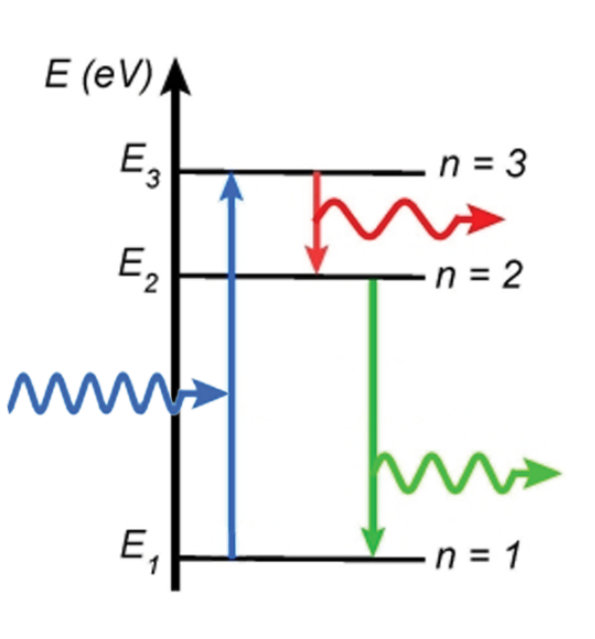
\includegraphics[width=0.5\textwidth]{Schema/nivenergie.png}
    \caption{Schéma des niveaux d'énergie d'un atome par des photons}
    \label{fig:niveau d'énergie}
\end{figure}
\section{Mise en équation du modèle à deux faisceaux}
Nous nous sommes intéressés au comportement des flux lumineux dans le modèle du transfert radiatif à deux faisceaux comme il a été décrit dans «~Fundamentals of atmosphere radiation~» \cite{textbook}.
Ce modèle composé d'un milieu exposé à deux flux de même orientation, mais de sens opposé, c’est-à-dire qu'il n'y a pas d'émission et de diffusion vers les côtés (fig:\ref{fig:modeledz}, seulement vers le haut ou le bas (selon une direction verticale seulement).
Les deux flux s'influencent l'un et l'autre par diffusion et sont atténués par absorption. 
En effet, nous ne prendrons pas en compte l'émission spontanée\footnote{l'émission spontanée est une émission qui a lieu un certain temps après l'absorption correspondante.}.
Une direction verticale signifie qu'il y a deux sens pour l'émission, elle n'est pas systématiquement dans un sens ou l'autre, en effet elle a une certaine probabilité de l'être\footnote{La probabilité qu'un photon suivant une trajectoire vers le haut soit diffusé par l'atome puis renvoyé vers le bas ou réciproquement sont respectivement nommé: $p_{{\uparrow}{\downarrow}}$ et $p_{{\downarrow}{\uparrow}}$.}. \par

\begin{figure}[H]
  \centering
  \includegraphics[width=0.5\textwidth]{Schema/schémarog1V2.jpg}
  \caption{Schéma de l'irradiance de la partie supérieure et inférieure d'un milieu par les flux respectifs ${F_{\downarrow}}$ et ${F_{\uparrow}}$, selon l'axe Oz orienté vers le bas.}
  \label{fig:photo}
\end{figure}
Les interactions considérées dans ce modèle sont donc:
\begin{itemize}
  \item L'\textbf{absorption} du photon par l'atome (Fig \ref{fig:photo}.*1)
  \item La \textbf{diffusion} du photon vers l'avant (Fig \ref{fig:photo}.*2)
  \item La \textbf{diffusion} du photon vers l'arrière (Fig \ref{fig:photo}.*3)
\end{itemize}

\begin{figure}
    \centering
    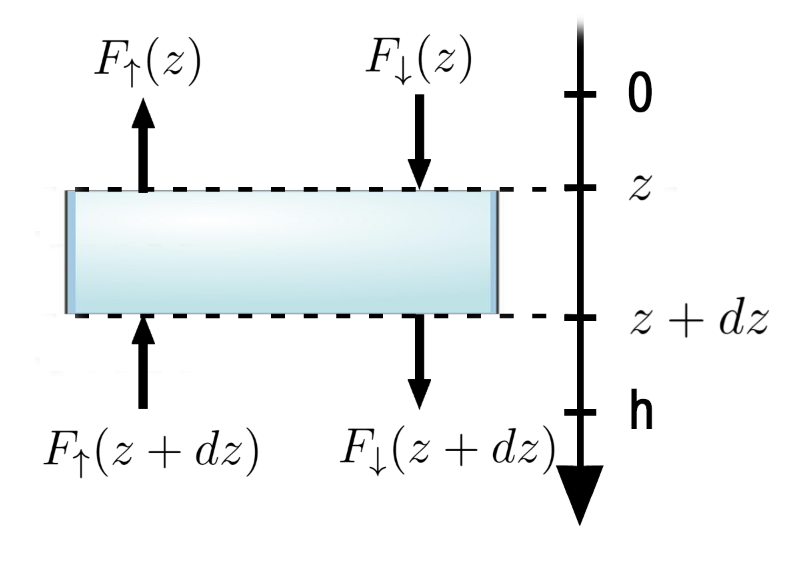
\includegraphics[width=0.5 \textwidth]{Schema/modele.png}
    \caption{Schéma inspiré de l'article de Bohren\cite{textbook}.}
    \label{fig:modeledz}
\end{figure}

Par conservation de l'énergie, nous pouvons exprimer les flux finaux $F_{\downarrow}(z+dz)$ et $F_{\uparrow}(z+dz)$, en fonction de:  $\kappa$ le coefficient d'absorption, $\beta$ le coefficient de diffusion en $m^{-1}$, $F_\downarrow$ le flux vers le bas et $p_{{\downarrow}{\uparrow}}$ la probabilité qu'un photon orienté vers le bas aille vers le haut.
En effet pour exprimer le flux descendant sortant en $z+dz$ il faut lister ce qui l'exprime:
\begin{itemize}
\item L'expression du flux descendant doit alimenter l'équation:
$F_{\downarrow}$
\item Il faut soustraire la partie absorbée de ce flux sur l'infime partie de z qui s'exprime avec le coefficient d'absorption, car ils ne font plus partie du flux descendant, soit: $\kappa dz F_{\downarrow}$.
\item Soustraire également (pour la même raison) l'expression des photons de ce flux diffusé vers le haut: $ \beta dz p_{\downarrow\uparrow} F_{\downarrow}(z+dz)$
\item Et enfin y ajouter la partie du flux montant qui alimente le flux descendant par sa diffusion :
$\beta dz p_{\uparrow\downarrow} F(z+dz)$
\end{itemize}
Ce qui nous donne l'équation générale du flux $F_{\downarrow}(z+dz)$:
\begin{equation}
    F_{\downarrow}(z+dz)=F_{\downarrow}(z)-\kappa dzF_{\downarrow}(z)-\beta dz p_{\downarrow\uparrow} F_{\downarrow}(z+dz)+\beta dz p_{\uparrow\downarrow} F_{\uparrow}(z+dz)
\end{equation}




\par Après avoir posé les principes de ce modèle, nous pouvons établir des équations, confirmées par Bohren; dont la caractérisation du comportement des flux descendants:
\begin{equation}
    \frac{dF_{\downarrow}}{dz}=-\kappa F_{\downarrow}-\beta p_{{\downarrow}{\uparrow}}F_{\downarrow} + \beta p_{{\uparrow}{\downarrow}}F_{\uparrow}
    \label{eq:fluxbas}
\end{equation}
\par
En réitérant le même raisonnement avec le flux montant ainsi que le sens de $-\widehat{u_z}$:

%avec $-\kappa F_{\downarrow}$ le terme correspondant à l'absorption et $\kappa$ le coefficient d'absorption en $m^{-1}$, $-\beta p_{{\downarrow}{\uparrow}}F_{\downarrow}$ le termes qui soustrait les photons remis vers l'arrière et $\beta$ le coefficient de diffusion en $m^{-1}$ et $\beta p_{{\uparrow}{\downarrow}}F_{\uparrow}$ le termes qui correspond aux photons remis vers l'arrière de $F_\uparrow$ qui va donc s'ajouter à $F_\downarrow$ \par
%Nous pouvons donc procéder identiquement avec le flux montant en faisant attention à l'orientation de $\widehat{u_z}$
\begin{equation}
    \frac{dF_{\uparrow}}{dz}=\kappa F_{\uparrow}+\beta p_{{\uparrow}{\downarrow}}F_{\uparrow} - \beta p_{{\downarrow}{\uparrow}}F_{\downarrow}
    \label{eq:fluxhaut}
\end{equation} \par
Pour s'affranchir des probabilités, nous allons définir $g,$ le paramètre d'asymétrie, qui sera compris entre -1 (diffusion totale vers l'arrière) et 1 (diffusion totale vers l'avant) tel que dans le cas isotrope \footnote{Un milieu isotrope est un milieu dont les propriétés physiques de celui-ci sont invariantes selon la direction, cela se traduit ici comme $p_{{\uparrow}{\downarrow}}=p_{{\downarrow}{\uparrow}}$.} :

\begin{equation}
    p_{{\uparrow}{\downarrow}}=p_{{\downarrow}{\uparrow}}=\frac{1-g}{2} 
    \label{eq:p}
\end{equation}
\begin{equation}
    p_{{\downarrow}{\downarrow}}=p_{{\uparrow}{\uparrow}}=\frac{1+g}{2}
\end{equation}\par
On définit également l'albédo de simple diffusion\footnote{L'albédo est une valeur comprise entre 0 et 1 qui s'obtient par le rapport entre le flux entrant et le flux réfléchi vers l'arrière%qui correspond à la capacité de diffusion d'un milieu, c'est à dire la capacité à disperser un flux. La simple diffusion correspond a renvoyer un flux seulement vers l'avant ou l'arrière
}
par :
\begin{equation}
    w=\frac{\beta}{\beta+\kappa}
    \label{eq:w}
\end{equation} \par

On remarque que, lorsque $w$ est nul, il n'y a pas de diffusion, tandis que, lorsque $w$ vaut 1, il n'y a pas d'absorption. Nous allons également appeler ${\tau}$ \textbf{l'épaisseur optique} tels que :
\begin{equation}
    d\tau=(\beta+\kappa)dz
    \label{eq:tau}
\end{equation}\par
\textbf{L'épaisseur optique} correspond à la distance parcourue dans le milieu par un flux, dans une unité particulière qui est le \textbf{libre parcours moyen}\footnote{C'est pourquoi deux faisceaux dont le coefficient $\beta$ et $\kappa$ auront parcouru la même distance à la sorti d'un milieu, mais pas forcément la même épaisseur optique}, c'est la distance moyenne parcourue par un photon pour que celui-ci est subi une interaction avec un atome.

En utilisant les équations \ref{eq:p}, \ref{eq:w} et \ref{eq:tau} avec \ref{eq:fluxbas} ou \ref{eq:fluxhaut} on obtient :

\begin{equation}
    \frac{dF_{\downarrow}}{d\tau}= (w-1)F_{\downarrow}-w \frac{1-g}{2} F_{\downarrow} + w \frac{1-g}{2} F_{\uparrow}
    \label{eq:fluxbas_final}
\end{equation}
\begin{equation}
    \frac{dF_{\uparrow}}{d\tau}=(1-w)F_{\uparrow}+w \frac{1-g}{2} F_{\uparrow} - w \frac{1-g}{2} F_{\downarrow}
    \label{eq:fluxhaut_final}
\end{equation}

\section{Analyse du système dynamique}
Maintenant que nous avons établi ce système d'équations différentielles couplées, nous allons utiliser les méthodes utilisées dans l'étude des systèmes dynamiques \cite{systemdynamique} pour obtenir le portrait de phase du système. Ces méthodes sont utilisées lorsqu'on dérive par rapport au temps, mais on peut également s'en servir lorsque nous dérivons par l'épaisseur optique. La première étape est de passer nos équations sous forme matricielle. Les équations \ref{eq:fluxbas_final} et \ref{eq:fluxhaut_final} donnent: 
\begin{equation}
    \begin{pmatrix}
        \dot{F_{\downarrow}} \\
        \dot{F_{\uparrow}}
    \end{pmatrix}
    =
%    \begin{pmatrix}
 %       w-1-w \frac{1-g}{2} &  w \frac{1-g}{2} \\
%        - w \frac{1-g}{2} & 1-w+w \frac{1-g}{2}
%    \end{pmatrix}
%    \begin{pmatrix}
%        F_{\downarrow}\\
 %       F_{\uparrow}
  %  \end{pmatrix}
   % =
    \begin{pmatrix}
        -1+w \frac{1+g}{2} &  w \frac{1-g}{2} \\
        - w \frac{1-g}{2} & 1-w \frac{1+g}{2}
    \end{pmatrix}
    \begin{pmatrix}
        F_{\downarrow}\\
        F_{\uparrow}
    \end{pmatrix}
    \label{eq:flux_matricielle}
\end{equation}\par
On va ensuite déterminer les vecteurs propres et valeurs propres de cette matrice. Les valeurs propres nous permettront de déterminer l'allure du diagramme de phase et les vecteurs propres nous permettront d'en déterminer les axes directeurs. Pour simplifier les équations, on pose:
\begin{equation}
    \begin{cases}
        a=1-w\left(\frac{1+g}{2}\right) \\
        b=w\left(\frac{1-g}{2}\right)
    \end{cases}
    \label{eq:abreviation}
\end{equation}\par
On obtient les valeurs propres et vecteurs propres suivant:
\begin{equation}
    \begin{cases}
        \lambda_1=\sqrt{a^2-b^2} & \overrightarrow{v_1}=
        \begin{pmatrix}
            b\\
            a+\lambda_1
        \end{pmatrix}\\
        \lambda_2=-\sqrt{a^2-b^2} & \overrightarrow{v_2}=
        \begin{pmatrix}
            a+\lambda_1\\
            b
        \end{pmatrix}
    \end{cases}
\end{equation}  \par
Nous avons vérifié que nos calculs étaient bons avec le site "wolframe alpha". On remarque que $a-b>0$ et donc que $\lambda_1$ et $\lambda_2$ sont des réels de signe opposé et donc que notre diagramme de phase aura un point selle en (0,0). 
\section{Traçage des graphes}
    Afin de comprendre comment les flux évoluent entre eux, nous avons tracé des graphes de phase pour plusieurs valeurs de $w$ et $g$. \par
    Pour cela, nous avons utilisé la fonction "streamplot" de la bibliothèque "mathplotlib". Cette fonction permet habituellement de tracer des vitesses en fonction des positions, pourtant comme le temps peut être considéré comme analogue à l'épaisseur optique, nous pouvons exploiter cette fonction. Cette fonction permet de tracer l'ensemble des solutions pour ce système dynamique, mais pas une solution particulière. Pour faire cela, nous nous sommes tournés vers la fonction \verb|"solve_ivp"| de la bibliothèque "scipy.integrate". Cette fonction prend en argument une fonction qui contient notre système dynamique, une valeur initiale et finale de $\tau$ et les valeurs initiales de $F_{\downarrow}$ et $F_{\uparrow}$ puis renvoie deux listes contenant les valeurs de $F_{\downarrow}$ et $F_{\uparrow}$ au cours de $\tau$ que l'on trace avec "plot" de "mathplotlib".
\begin{figure}[H]
    \centering
    \begin{subfigure}{0.59\textwidth}
      \centering
      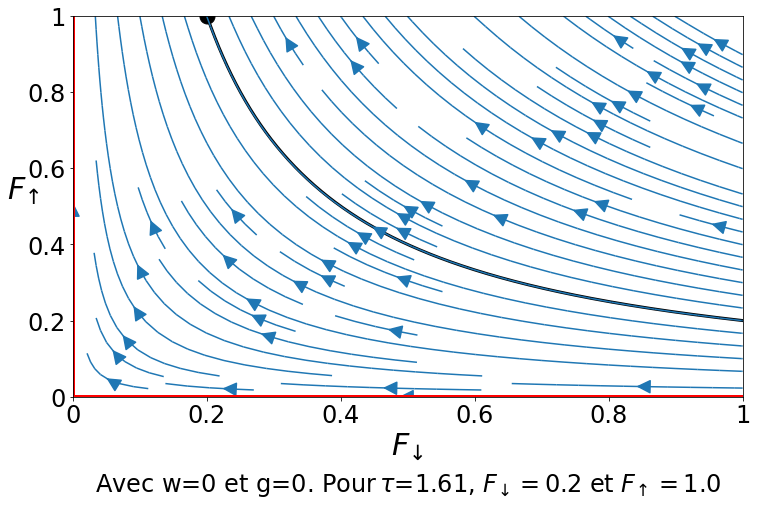
\includegraphics[width=1\textwidth]{Graphe/Figure W=0.png}
      \captionsetup{width=.85\textwidth}
      \caption{}  
      \label{fig:Sub_Graphe_W=0}
    \end{subfigure}%
    \begin{subfigure}{0.3\textwidth}
        \centering
        \captionsetup{width=1.4\textwidth}
        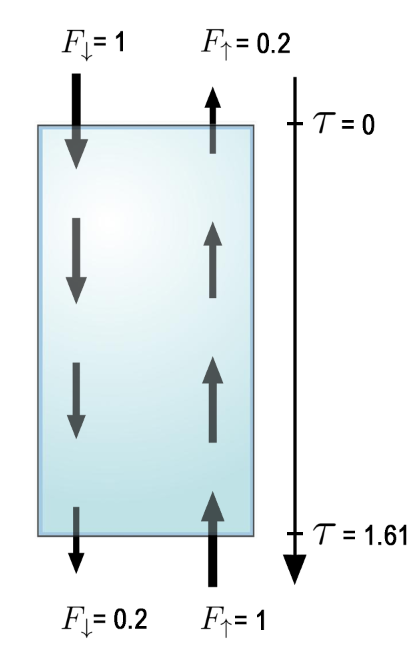
\includegraphics[width=1\textwidth]{Schema/W=0.png}
        \caption{} 
        \label{fig:Sub_Schema_W=0}
    \end{subfigure}
    \caption{Comportement des flux lorsque $w=0$.} 
    \label{fig:W=0}
    \justifying \noindent
    (a) Graphe de $F_{\uparrow}$ en fonction de $F_{\downarrow}$. Le schéma ne dépend pas de $g$ quand $w=0$. Les vecteurs propres sont représentés en rouge, ils sont confondus avec les axes.\\ (b) Schéma du comportement des flux lumineux de la courbe noire, la taille des flèches est proportionnelle à l'intensité du flux lumineux.
\end{figure} %w=0
\par 
Nous avons maintenant des graphiques qui représentent l'évolution des flux montants en fonction des flux descendants. Ces graphiques sont des champs vectoriels dont une courbe représente tous les couples de flux montant et descendant en fonction de l'épaisseur optique pour une condition initiale. Les flèches représentent la direction du vecteur quand $\tau$ augmente. La courbe noire représente la solution particulière du système dynamique qui est représenté sur le schéma à droite (b) et le point noir l'état du système pour un $\tau$ final fixé. 

Dans le cas où w=0 (Fig: \ref{fig:W=0}), cela signifie que l'albédo est nul, c'est-à-dire qu'il n'y a pas de diffusion, nous retrouvons alors la loi de Beer-Lambert. La totalité du flux rentrant est donc égale au flux sortant additionné à celui absorbé dans le milieu pour chaque faisceau.
%Les flèches sur la Fig \ref{fig:Sub_Graphe_W=0} indiquent le sens de croissance de l'épaisseur optique de chaque flux.
Prenons l'exemple de la courbe noire: initialement avec un flux vers le bas et vers le haut respectivement de 1 et 0.2, en augmentant l'épaisseur optique jusqu'à 1.61, nous constatons que le flux est absorbé de manière exponentielle jusqu'à atteindre un flux montant de 1 et descendant\footnote{flux montant signifie flux vers le haut, et réciproquement pour le flux descendant} de 0.2.
Le cas souvent observé à cause de notre soleil est avec initialement $F_{\downarrow}=1$ et $F_{\uparrow}=0$, nous constatons que lorsque $\tau$ augmente le flux montant est inchangé mais le flux descendant tend vers 0.


\begin{figure}[H]
    \centering
    
    \begin{subfigure}{0.625\textwidth}
      \centering
      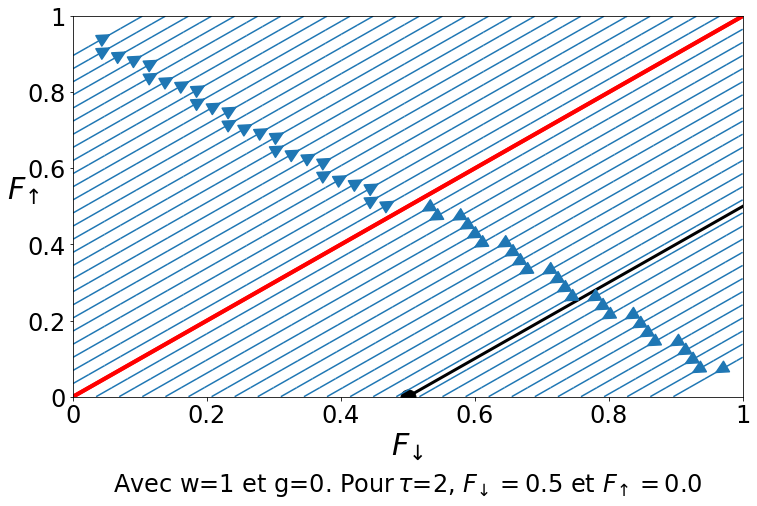
\includegraphics[width=1\textwidth]{Graphe/Figure W=1.png}
      \captionsetup{width=.85\textwidth}
      \caption{} 
      \label{fig:Sub_Graphe_W=1}
    \end{subfigure}
    \begin{subfigure}{0.305\textwidth}
        \centering
        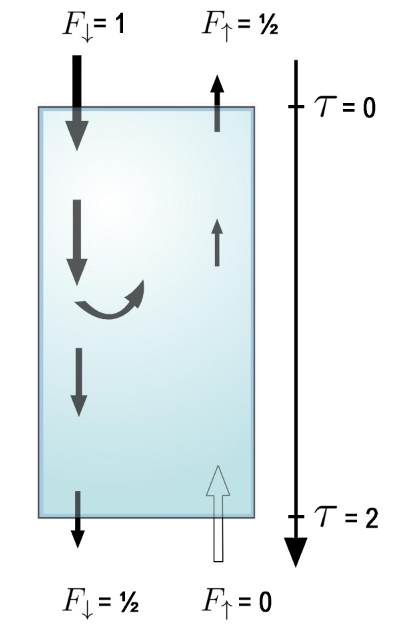
\includegraphics[width=1\textwidth]{Schema/W=1.png}
        \captionsetup{width=1.2\textwidth}
        \caption{} 
        \label{fig:Sub_Schema_W=1}
    \end{subfigure}
    \caption{Comportement des flux lorsque $w=1$.}
    \justifying \noindent
    (a) Graphe de $F_{\uparrow}$ en fonction de $F_{\downarrow}$. Le schéma ne dépend pas de g lorsque $w=1$. Les vecteurs propres sont représentés en rouge, ils sont confondus entre eux. \\(b) : Schéma du comportement des flux lumineux de la courbe noire, la taille des flèches est proportionnelle à l'intensité du flux lumineux.
    \label{fig:W=1}
\end{figure} %w=1
Dans le cas où $w=1$, $\beta$ a la même valeur partout mais seul les conditions initiales changent. L'absorption est nulle et le portrait de phase est montré sur la figure \ref{fig:W=1}.
Plus la droite se rapproche de l'axe des vecteurs propres, plus l'effet de diffusion s'intensifie jusqu'à atteindre une diffusion complète. 
Concernant la nouvelle courbe noire, nous pouvons constater que les flux initiaux sont de 0.5 en ordonnée et 1 en abscisse.
La seule manière d'obtenir ce cas de figure avec un flux montant final nul est que la moitié du flux descendant soit ré-émis vers l'arrière pour devenir du flux montant et que
l'autre moitié poursuit sa trajectoire, car il n'y a pas d'absorption (Fig: \ref{fig:Sub_Schema_W=1}).

\begin{figure}[H]
    \centering
    \begin{subfigure}{0.63\textwidth}
      \centering
      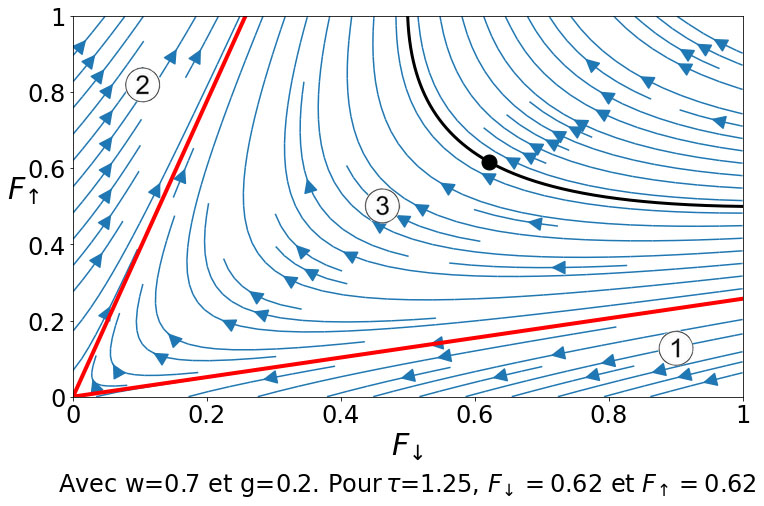
\includegraphics[width=1\textwidth]{Graphe/Figure W=quelque et g quelquonque.png}
      \captionsetup{width=.85\textwidth}
      %\caption{Graphe de $F_{\uparrow}$ en fonction de $F_{\downarrow}$ Le choix de w=0.7 et g=0.2 est arbitraire pour représenter un cas quelconque. Sont représentés en rouge les vecteurs propres.}
      \caption{} 
      \label{fig:Sub_Graphe_W=0.7}
    \end{subfigure}
    %
    \begin{subfigure}{0.32\textwidth}
        \centering
        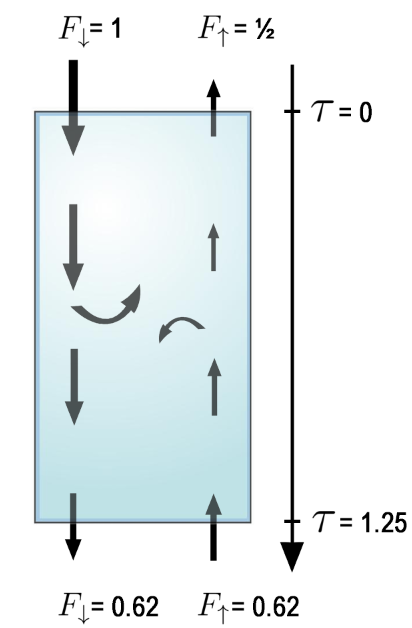
\includegraphics[width=1\textwidth]{Schema/G=0.2.png}
        \captionsetup{width=1.2\textwidth}
        %\caption{Schéma du comportement des flux lumineux\newline}
        \caption{} 
        \label{fig:Sub_Schema_W=0.7}
    \end{subfigure}
    \caption{Comportement des flux lorsque $w=0.7$ et $g=0.2$.}
    \label{fig:W=0.7}
    \justifying \noindent
    (a) Graphe de $F_{\uparrow}$ en fonction de $F_{\downarrow.}$ Le choix de $w=0.7$ et $g=0.2$ est arbitraire pour représenter un cas quelconque. Les vecteurs propres sont représentés en rouge.\\(b)Comportement des flux lorsque $w=0.7$ et $g=0.2$ pour la courbe noire, la taille des flèches est proportionnelle à l'intensité du flux lumineux.
\end{figure} %Cas quelquonque

Lorsque l'on prend un cas quelconque, l'interprétation est plus complexe, en effet ici tous les phénomènes vus précédemment sont présents avec les proportions variables, par exemple comme g=0.7 dans ce cas $p_{{\uparrow}{\downarrow}}$ et $p_{{\downarrow}{\uparrow}}$ sont de $\frac{1-0.7}{2}=0.15$.\par
Nous distinguons trois zones sur ce graphique (Fig: \ref{fig:Sub_Graphe_W=0.7}). Dans la zone comprise entre le vecteur propre et l'axe des abscisses (zone \textcircled{\small1}), nous constatons que tous les flux montants tendent vers 0, cela est dû au fait que pour un flux $F_{\downarrow}$ de 1, si $F_{\uparrow}$ est inférieur ou égal à 0.25 alors il tendra vers 0 en augmentant l'épaisseur optique. La composante de  $F_{\downarrow}$ qui est diffusée vers l'arrière ne permet pas d'alimenter le flux montant à cause de l'absorbance du milieu, elle ne peut donc pas nourrir le flux opposé s'il est inférieur à 0.25.
L'interprétation de la zone \textcircled{\small2} suit le même raisonnement, mais avec $\tau$ inversé. 
\par
On peut prendre comme exemple la courbe noire pour expliquer la zone \textcircled{\small3}. Elle représente la solution particulière avec un flux initial montant de 0.5 et descendant de 1. Lorsque $\tau$ = 1.25, $F_{\downarrow}$ et  $F_{\uparrow}$ ont tout deux comme valeur 0.62. 

\subsection{Calcul de l'angle entre les vecteurs propres}
Pour calculer l'angle entre les vecteurs propres, nous allons exploiter les formules du produit scalaire. On prend $V_1=\begin{pmatrix}
    x_{1}\\
    y_{1}
\end{pmatrix}$ et $V_2=\begin{pmatrix}
    x_{2}\\
    y_{2}
\end{pmatrix}$
\begin{equation}
    \overrightarrow{V_1}.\overrightarrow{V_2}=||\overrightarrow{V_1}||*||\overrightarrow{V_2}||*cos(\theta)=x_{1}*x_{2}+y_{1}*y_{2}
\end{equation}
\begin{equation}
    \sqrt{x_{1}^2+y_{1}^2}*\sqrt{x_{2}^2+y_{2}^2}*cos(\theta)=x_{1}*x_{2}+y_{1}*y_{2}
\end{equation}
\begin{equation}
    \theta=cos^{-1}\left(\frac{x_{1}*x_{2}*\sqrt{x_{1}^2+y_{1}^2}*\sqrt{x_{2}^2+y_{2}^2}*+y_{1}*y_{2}*\sqrt{x_{1}^2+y_{1}^2}*\sqrt{x_{2}^2+y_{2}^2}}{x_{1}^2 x_{2}^2 + x_{1}^2 y_{2}^2 + y_{1}^2 x_{2}^2 + y_{1}^2 y_{2}^2}\right)
\end{equation}
Comme on se place dans le cas isotrope où $x_{1}=y_{2}=b$ et $y_{1}=x_{2}=a+\lambda_1$ on obtient 
\begin{equation}
    \theta=cos^{-1}\left(\frac{2*x_{1}*y_{1}}{x_{1}^2 + y_{1}^2}\right)=cos^{-1}\left(\frac{b}{a} \right)=cos^{-1}\left(\frac{w\left(\frac{1-g}{2}\right)}{1-w\left(\frac{1+g}{2}\right)}\right)
    \label{eq:angle}
\end{equation}
C'est pourquoi dans les cas extrêmes on à:
\begin{itemize}
    \item Lorsque $w=0$ \\
$\theta=cos^{-1}\left(0\right)=\frac{\pi}{2}$ ce qui suis bien le graphique \ref{fig:Sub_Graphe_W=0}.
    \item lorsque $w=1$
    \\$\theta=cos^{-1}\left(\frac{\frac{1-g}{2}}{1-\left(\frac{1+g}{2}\right)}\right)=0$ ce qui suis bien le graphique \ref{fig:Sub_Graphe_W=1}
\end{itemize}
En résolvant avec python l'équation \ref{eq:angle} l'angle est de $\theta=1.10\unit{rad}=63.55^\circ$ pour $w=0.7$ et $g=0.2$
%Nous constatons que le flux descendant est fortement atténué et le flux montant est légèrement augmenté pour atteindre tous deux 0.62 comme schématisé sur la fig(\ref{fig:Sub_Schema_W=0.7}).

\subsection{Milieu non isotrope}
Le milieu étudié précédemment a jusque là été considéré comme isotrope, les propriétés du milieu étant désormais mis en évidence nous allons étudier un milieu qui ne répond pas à l'égalité de l'isotropie. En reprenant les calcule, on trouve que

\begin{equation}
    \begin{pmatrix}
        \dot{F_{\downarrow}}\\
        \dot{F_{\uparrow}}
    \end{pmatrix}=
    \begin{pmatrix}
        -1+wp_{{\downarrow}{\downarrow}} & wp_{{\uparrow}{\downarrow}} \\
         -w p_{{\downarrow}{\uparrow}} & 1-wp_{{\uparrow}{\uparrow}} 
    \end{pmatrix}
    \begin{pmatrix}
        F_{\downarrow}\\
        F_{\uparrow}
    \end{pmatrix}
    \label{eq:matrice non iso}
\end{equation}\par
Sur la figure \ref{fig:non.iso} nous pouvons constater que l'allure globale des courbes suivent le même modèle que dans le modèle isotrope avec également $w=0.7$ (fig: \ref{fig:W=0.7}).
La différence drastique est le coefficient des vecteurs propres.
\begin{figure}[H]
    \centering
    \begin{subfigure}{0.61\textwidth}
      \centering
      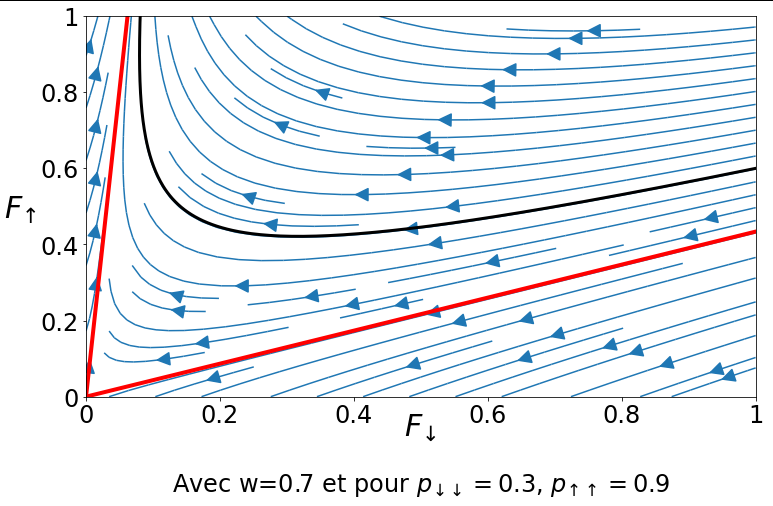
\includegraphics[width=1\textwidth]{Graphe/non.iso.png}
      \captionsetup{width=.85\textwidth}
      \caption{} 
      \label{graph:non.iso}
    \end{subfigure}
    \begin{subfigure}{0.335\textwidth}
        \centering  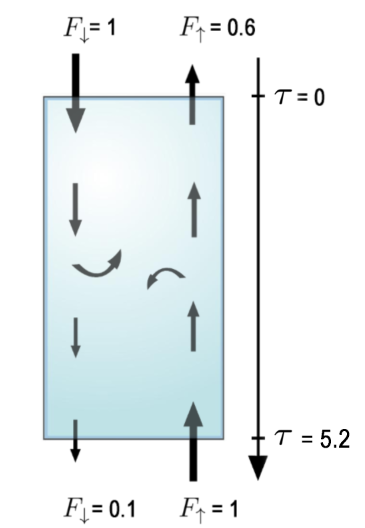
\includegraphics[width=1\textwidth]{Schema/non.iso.png}
        \captionsetup{width=1\textwidth}
        \caption{} 
        \label{schéma:non.iso}
    \end{subfigure}
    \caption{Comportement des flux dans un milieu non isotrope pour $P_{\uparrow\uparrow}=0.9$ et $P_{\downarrow\downarrow}=0.3$.}
    \label{fig:non.iso}
    \justifying \noindent
    (a) Graphe de $F_{\uparrow}$ en fonction de $F_{\downarrow}$ dans un milieu non isotrope . Les vecteurs propres sont représentés en rouge.\\(b)Comportement des flux dans ce même milieu pour la courbe noire, la taille des flèches est proportionnelle à l'intensité du flux lumineux.
\end{figure}


\section{Conservation du volume}
On sait que dans un champ de vitesse, si la divergence d'un champ vectoriel est nulle, cela indique que le volume à l'intérieur d'une région donnée reste constant. La divergence peut s'exprimer comme:
\begin{equation}
    div \overrightarrow v =\frac{\partial {v_x}}{\partial x}+\frac{\partial {v_y}}{\partial y}
\end{equation}
Or $\tau$ est analogue au temps et l’on peut donc dire que $\begin{pmatrix}
        \dot{F_{\downarrow}} \\
        \dot{F_{\uparrow}}
    \end{pmatrix}$ s'exprime comme un vecteur vitesse. 
\subsection{Cas Isotope}    
    En utilisant les équations \ref{eq:flux_matricielle} et \ref{eq:abreviation} on obtient:
    \begin{equation}
        div\begin{pmatrix}
        \dot{F_{\downarrow}} \\
        \dot{F_{\uparrow}}
    \end{pmatrix}=-a+a=0
    \end{equation}
La divergence de $\begin{pmatrix}
        \dot{F_{\downarrow}} \\
        \dot{F_{\uparrow}}
    \end{pmatrix}$ est nulle donc le volume se conserve dans l'espace des phases. On remarque que la divergence est égale à la trace de la matrice de l'équation \ref{eq:flux_matricielle}. La conservation du volume implique qu'un point dans le volume initial sera contenu dans le volume final, ce qui simplifie les calculs.

    
\begin{figure}[H]
    \centering
    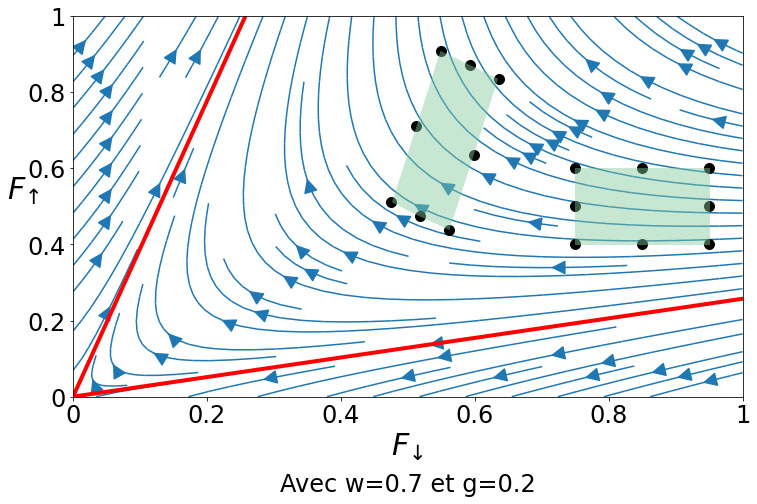
\includegraphics[width=0.7\textwidth]{Graphe/Figure Conservation du volume.png}
    \caption{Graphique de $F_{\uparrow}$ en fonction de $F_{\downarrow}$ représentant la conservation de la surface (les points sont des valeurs calculées pour deux valeurs de $\tau$ espacer de 1.25).}
    \label{fig:volume}
\end{figure}    

Comme le montre le graphique \ref{fig:volume}, les surfaces des deux carrés verts n'ont pas la même forme, mais possèdent le même volume. Un point contenu dans la surface d'une des formes pour un certain $\tau$ sera contenu dans l'autre surface pour le $\tau$ correspondant, il restera forcément dans cette même surface après la transformation par la matrice de l'équation \ref{eq:flux_matricielle}.
\subsection{Cas Non-Isotrope}
Dans le cas non isotrope, on trouve à partir de \ref{eq:matrice non iso} que: 
\begin{equation}
    div\begin{pmatrix}
        \dot{F_{\downarrow}} \\
        \dot{F_{\uparrow}}
    \end{pmatrix}=-1+wp_{{\downarrow}{\downarrow}} +1-wp_{{\uparrow}{\uparrow}} = w(p_{\downarrow\downarrow}-p_{\uparrow\uparrow})
\end{equation}\par
On remarque que $div\begin{pmatrix}\dot{F_{\downarrow}} \\ \dot{F_{\uparrow}}\end{pmatrix}=0$ si et seulement si $p_{{\downarrow}{\downarrow}}=p_{{\uparrow}{\uparrow}}$ ce qui reviendrait à se placer dans le cas isotrope (ce qui est possible de voir visuellement à partir de la fig: \ref{fig:non-volume}), de plus le volume augmente si $p_{\downarrow\downarrow}>p_{\uparrow\uparrow}$ et diminue si $p_{\downarrow\downarrow}<p_{\uparrow\uparrow}$. 

\begin{figure}[H]
    \centering
    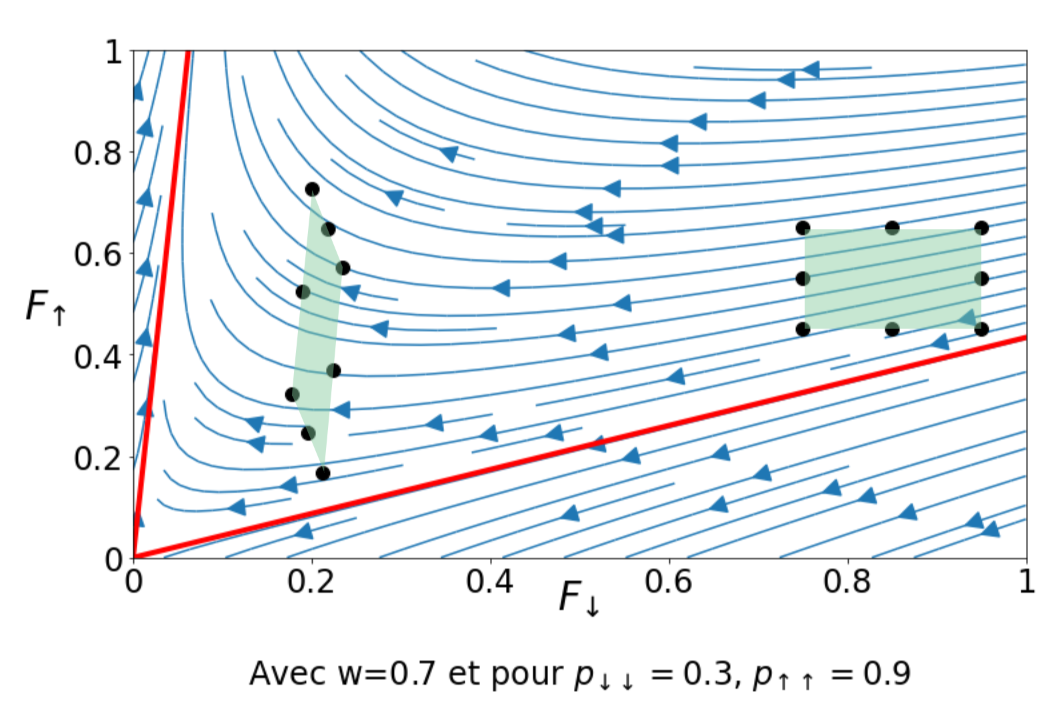
\includegraphics[width=0.7\textwidth]{Graphe/non.cons.png}
    \caption{Graphique de $F_{\uparrow}$ en fonction de $F_{\downarrow}$ représentant la non-conservation de la surface (les points sont des valeurs calculées pour deux valeurs de $\tau$ espacer de 2).}
    \label{fig:non-volume}
\end{figure}

\section{Modèle aux ordres supérieurs}
On va essayer de généraliser le modèle a 2 faisceaux en rajoutant deux faisceaux latéraux %inserer schema
\begin{equation}
    \frac{dF_{\downarrow}}{dz}=-\kappa F_{\downarrow}-\beta (p_{{\downarrow}{\uparrow}}+p_{{\downarrow}{\leftarrow}}+p_{{\downarrow}{\rightarrow}})F_{\downarrow} + \beta( p_{{\uparrow}{\downarrow}}F_{\uparrow}+p_{{\leftarrow}{\downarrow}}F_{\leftarrow}+p_{{\rightarrow}{\downarrow}}F_{\rightarrow})
\end{equation} \par car $p_{{\downarrow}{\uparrow}}+p_{{\downarrow}{\leftarrow}}+p_{{\downarrow}{\rightarrow}}+p_{{\downarrow}{\downarrow}}=1$, on peut donc écrire:
\begin{equation}
    \frac{dF_{\downarrow}}{dz}=(-\kappa -\beta +\beta p_{{\downarrow}{\downarrow}})F_{\downarrow}+ \beta( p_{{\uparrow}{\downarrow}}F_{\uparrow}+p_{{\leftarrow}{\downarrow}}F_{\leftarrow}+p_{{\rightarrow}{\downarrow}}F_{\rightarrow})   
\end{equation}\par
On peut étendre cela aux trois autres équations en faisant attention au signe et à l'axe selon lequel on dérive.
\begin{equation}
    \frac{dF_{\uparrow}}{dz}=(\kappa +\beta -\beta p_{{\uparrow}{\uparrow}})F_{\uparrow}- \beta( p_{{\downarrow}{\uparrow}}F_{\downarrow}+p_{{\rightarrow}{\uparrow}}F_{\rightarrow}+p_{{\leftarrow}{\uparrow}}F_{\leftarrow})
\end{equation}
\begin{equation}
    \frac{dF_{\leftarrow}}{dy}=(-\kappa -\beta +\beta p_{{\leftarrow}{\leftarrow}})F_{\leftarrow}+ \beta( p_{{\rightarrow}{\leftarrow}}F_{\rightarrow}+p_{{\uparrow}{\leftarrow}}F_{\uparrow}+p_{{\downarrow}{\leftarrow}}F_{\downarrow})
\end{equation}
\begin{equation}
    \frac{dF_{\rightarrow}}{dy}=(\kappa +\beta -\beta p_{{\rightarrow}{\rightarrow}})F_{\rightarrow}- \beta( p_{{\leftarrow}{\rightarrow}}F_{\leftarrow}+p_{{\downarrow}{\rightarrow}}F_{\downarrow}+p_{{\uparrow}{\rightarrow}}F_{\uparrow})
\end{equation}\par
En posant ces équations sous forme matricielle $\dot{X}=AX$ et $h=-\kappa -\beta$, on obtient:
\begin{equation}
    \begin{pmatrix}
        \frac{dF_{\downarrow}}{dz}\\[4pt]
        \frac{dF_{\uparrow}}{dz}\\[4pt]
        \frac{dF_{\leftarrow}}{dy}\\[4pt]
        \frac{dF_{\rightarrow}}{dy}
    \end{pmatrix}=
    \begin{pmatrix}
        h+\beta p_{{\downarrow}{\downarrow}} & \beta p_{{\uparrow}{\downarrow}} & \beta p_{{\leftarrow}{\downarrow}} & \beta p_{{\rightarrow}{\downarrow}} \\
         -\beta p_{{\downarrow}{\uparrow}} & -h-\beta p_{{\uparrow}{\uparrow}} &  -\beta p_{{\leftarrow}{\uparrow}} &  -\beta p_{{\rightarrow}{\uparrow}} \\
        \beta p_{{\downarrow}{\leftarrow}} & \beta p_{{\uparrow}{\leftarrow}} & h +\beta p_{{\leftarrow}{\leftarrow}} & \beta p_{{\rightarrow}{\leftarrow}} \\
         -\beta p_{{\downarrow}{\rightarrow}} &  -\beta p_{{\uparrow}{\rightarrow}} &  -\beta p_{{\leftarrow}{\rightarrow}} & -h -\beta p_{{\rightarrow}{\rightarrow}} 
    \end{pmatrix}
    \begin{pmatrix}
        F_{\downarrow}\\
        F_{\uparrow}\\
        F_{\leftarrow}\\
        F_{\rightarrow}
    \end{pmatrix}
    \label{eq:Flux Matriciel 4 direction}
\end{equation}\par
On remarque que  $div(\dot{X})=tr(A)$ et que   $tr(A)=0$ si et seulement si $p_{{\rightarrow}{\rightarrow}}=p_{{\leftarrow}{\leftarrow}}$ et $p_{{\downarrow}{\uparrow}}=p_{{\uparrow}{\downarrow}}$. \par On en conclut donc que le volume se conserve seulement dans le cas isotrope, ce qui est en accord avec les résultats précédents.\par
    
On généralise au cas avec n dimensions avec $h=-\kappa -\beta$.

\begin{equation}
    \begin{pmatrix}
         \frac{dF_{1}}{dx_1}\\[4pt]
        \frac{dF_{2}}{dx_1}\\
        \vdots \\
        \frac{dF_{2n-1}}{dx_n}\\[4pt]
        \frac{dF_{2n}}{dx_n}
    \end{pmatrix}=
    \begin{pmatrix}
        h+\beta p_{{1},{1}} & \beta p_{{2},{1}} & \hdots & \beta p_{{2n-1},{1}} & \beta p_{{2n},{1}}\\
        -\beta p_{{1},{2}} & -h-\beta p_{{2},{2}} & \hdots & -\beta p_{{2n-1},{2}} & -\beta p_{{2n},{2}}\\
        \vdots & \vdots & \ddots & \vdots & \vdots \\\
        \beta p_{{1},{2n-1}} & \beta p_{{2},{2n-1}} & \hdots & h+\beta p_{{2n-1},{2n-1}} & \beta p_{{2n},{2n-1}}\\
        -\beta p_{{1},{2n}} & -\beta p_{{2},{2n}} & \hdots & -\beta p_{{2n-1},{2n}} & -h-\beta p_{{2n},{2n}}
    \end{pmatrix}
    \begin{pmatrix}
        F_{1}\\
        F_{2}\\
        \vdots \\
        F_{2n-1}\\
        F_{2n}
    \end{pmatrix}
    \label{eq:flux_matriciel_n_dim}
\end{equation}\par
On a toujours $div(\dot{X})=tr(A)$ et que $tr(A)=0$ si et seulement si $\forall n$, $p_{{2n-1},{2n-1}}=p_{{2n},{2n}}$. La trace étant nulle, la divergence l'est aussi.\par Nous pouvons généraliser qu'à l'ordre N, le volume se conserve si et seulement si le milieu est isotrope.

\section{Variation du portrait de phase avec la fréquence}
Nous avons vu précédemment que les interactions photons-milieu suivent des lois, elles-mêmes régies par des coefficients d'absorption et de diffusion.
Ces coefficients dépendent de la nature du milieu, mais aussi la longueur d'onde du flux lumineux étudié, c'est pourquoi après avoir étudié les cas théoriques, nous allons étudier la variation des flux $F_\downarrow$ et $F_\uparrow$ dans l'eau et dans l'air en fonction de deux longueurs d'ondes: 450nm (bleu) et 675nm (rouge).


%\subsection{Cas théoriques}
%En étudiant des valeurs particulières des coefficients de deux rayons de couleur bleu et rouge, nous pourrons mettre en évidence des cas théoriques.
%Dans un premier temps avec des coefficients d'absorption identique entre les deux flux (fig: \ref{}), puis avec des coefficients d'émission identique (fig: \ref{}).



\subsection{Variation dans l'eau}


%On constate sur la figure \ref{subfig:graph.eau} que toutes les courbes qui partent de l'extrémité du graphe arrivent à la même extrémité du graphe, mais qu'elles ne suivent pas le même chemin pour y arriver. Sur la figure \ref{subfig:Tau.long}, on voit que les différentes longueurs d'onde se comportent différemment dans l'eau. Les longueurs d'onde plus grandes que ~525nm ne dépassent pas un $\tau=1$ alors qu’en dessous de 525nm, plus la longueur d'onde est faible moins elle a d'interaction sur une même distance. C'est pour cela que dès que l'on plonge un peu on ne voit que du bleu.
On remarque que dans l'eau les différentes longueurs d'onde n'auront pas la même intensité pour une profondeur identique (fig: \ref{subfig:graph.eau}). Cela s'explique par le fait que chaque longueur d'onde possède un libre parcours moyen différent dans l'eau, alors elles ont donc des épaisseurs optiques différentes pour une même distance parcourue. En comparant la figure \ref{subfig:Tau.long} et \ref{subfig:eau beta kappa} on constate que l'allure de la courbe de $\tau_{final}$ est très similaire à celle de la courbe de $\kappa$. Cela est dû au fait que $\tau=(\beta+\kappa)z$ et comme $\beta<<\kappa$ on obtient alors une allure de courbe quasiment identique. \par
L'interprétation de la figure \ref{subfig:graph.eau} peut se faire de plusieurs manières à l'aide de la figure \ref{subfig:fréquence_eau}. Si l'on regarde simplement $F_{\downarrow}$ alors lorsque $z=50$, la longueur d'onde majoritaire est le bleu tandis qu'il reste bien moins de rouge et de vert car leur valeur de $\bar F_{\downarrow}$ est plus petite. Le plongeur représenté sur la figure \ref{subfig:fréquence_eau} observera donc bien plus de bleu que d'autres couleurs.\par
On peut également comprendre de quelle couleur devrait être le flux montant à 50m pour obtenir du blanc à la surface de l'eau $F_{\uparrow}$.
En effet, pour avoir de la lumière blanche en sortie il faut que quand $\tau=0$, toutes les longueurs d'onde soient à la même intensité. Pour cela il faudra partir avec beaucoup plus de rouge que de bleu (représenté en bas à droite sur la fig: \ref{subfig:fréquence_eau}). Ces valeurs se lisent sur l'axe $F_{\uparrow}$ au point où les courbes se finissent. 

\begin{figure}[H]
    \centering
    \begin{subfigure}{0.48\textwidth}
        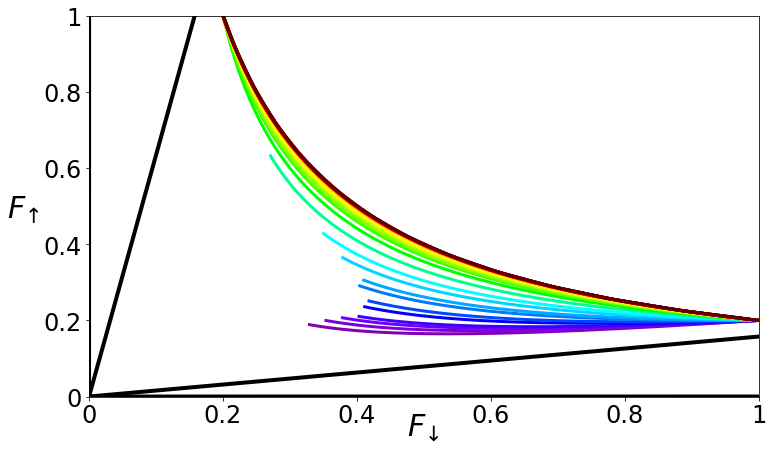
\includegraphics[width=1 \textwidth]{Graphe/eau.png}
        \caption{}
        \label{subfig:graph.eau}
    \end{subfigure}
    \begin{subfigure}{0.48\textwidth}
        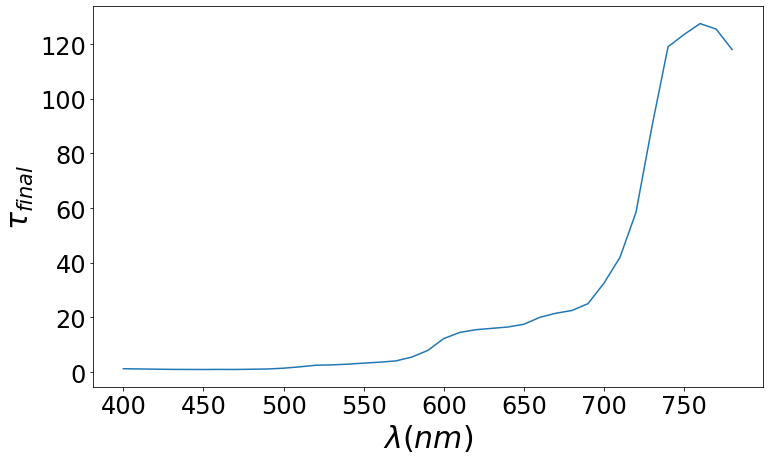
\includegraphics[width=1 \textwidth]{Graphe/Tau en fonction longeur d'onde.png}
        \caption{}
        \label{subfig:Tau.long}
    \end{subfigure}
    \begin{subfigure}{0.55\textwidth}
        \includegraphics[width=1 \textwidth]{Graphe/Béta_kappa.png}
        \caption{}
        \label{subfig:eau beta kappa}
    \end{subfigure}
    \begin{subfigure}{0.39\textwidth}
        \includegraphics[width=1 \textwidth]{Schema/fréquence_eau.png}
        \caption{}
        \label{subfig:fréquence_eau}
    \end{subfigure}
    \caption{Comportement des différentes longueurs d'onde dans l'eau}
    \justifying \noindent
    Les coefficients d'absorption et de diffusion ont été extraits de l'article Smith, 1981 \cite{Smith:81}. \newline
    (a) Graphe $F_{\uparrow}$ en fonction de $F_{\downarrow}$. Toutes les courbes ont (1; 0.2) comme point de départ et sont tracées sur une profondeur de 50m. Les vecteurs propres associés au $w$ de la longueur d'onde 400nm (min) est visible. Les vecteurs propres de la longueur d'onde 780nm (max) sont quasiment confondus avec les axes. Les couleurs des courbes sont issues du calcul des valeurs RGB associées aux longueurs d'onde.\newline
    (b) Graphe de la longueur d'onde en fonction du $\tau$ final de la figure a. 
    \\(c) Variation de \textcolor{red}{$\beta$ (en rouge)} et \textcolor{blue}{$\kappa$ (en bleu)} en fonction de la longueur d'onde.
    \\(d) Schéma représentant les fréquences et leurs proportions dans l'eau avec les valeurs de la figure \ref{subfig:graph.eau}, la taille des flèches est proportionnelle à l'intensité des flux
    \label{fig:longeur_eau}
\end{figure}







\subsection{Variation dans l'air}
\begin{figure}[H]
    \centering
    \begin{subfigure}{0.49\textwidth}
        \includegraphics[width=1 \textwidth]{Schema/schéma.rayleigh.png}
        \caption{}
        \label{subfig:Rayleigh}
    \end{subfigure}
    \begin{subfigure}{0.49\textwidth}
        \includegraphics[width=1 \textwidth]{Schema/couché_soleil.png}
        \caption{}
        \label{subfig:soleil}
    \end{subfigure}
    \caption{La diffusion de Rayleigh}
    \label{fig:atm}
    \justifying \noindent
     (a) Schéma explicatif du modèle de diffusion de Rayleigh de flux bleu et rouge, la taille des flèches est proportionnelle à l'intensité des flux.
    \\(b) Schéma de l'impact de la diffusion de Rayleigh dans la couleur perçue du soleil, la taille des flèches est proportionnelle à l'intensité des flux.
\end{figure}

Dans l'air c'est la diffusion de Rayleigh \cite{cours_Rayleigh} qui est le mécanisme prépondérant dans le visible. Le bleu est plus diffusé que le rouge dans toutes les directions de l'espace. Le faisceau bleu perd donc plus de flux que le faisceau rouge dans la direction incidente (voir fig: \ref{fig:atm}). Cela se traduit par un coefficient d'absorption plus fort pour le bleu que pour le rouge dans le modèle à deux faisceaux. Plus précisément on a:

\begingroup{}
\large
\begin{equation}
    \begin{matrix}
        \kappa_{bleu}=\left ( \dfrac{\lambda_{rouge}}{\lambda_{bleu}}\right )^4 *\kappa_{rouge} & et & \beta_{bleu}=\left ( \dfrac{\lambda_{rouge}}{\lambda_{bleu}}\right )^4 *\beta_{rouge} & \Rightarrow & w_{rouge}=w_{bleu}
    \end{matrix}
\end{equation}
\endgroup{}

Les portraits de phase du bleu et du rouge sont donc les mêmes dans l'air (voire fig: \ref{fig:air}).\par

Par contre l'épaisseur optique du faisceau bleu est plus grande que celle du faisceau rouge. $\bar{\tau}_{bleu}=\left ( \dfrac{\lambda_{rouge}}{\lambda_{bleu}}\right )^4 *\bar{\tau}_{rouge}$. C'est ce que nous observons dans la figure \ref{fig:air}. La cas \textcircled{\small A} de la figure \ref{fig:air} montre que le flux \textcolor{red}{$F_{\downarrow}$ rouge} est supérieur au flux \textcolor{blue}{$F_{\downarrow}$ bleu}. Au début $F_{\downarrow 0 \, bleu}=F_{\downarrow 0 \, rouge}$. On retrouve ainsi le fait que le coucher du soleil apparaisse rouge (figure \ref{subfig:soleil}).

\begin{figure}[H]
    \centering
    \begin{subfigure}{0.645\textwidth}
        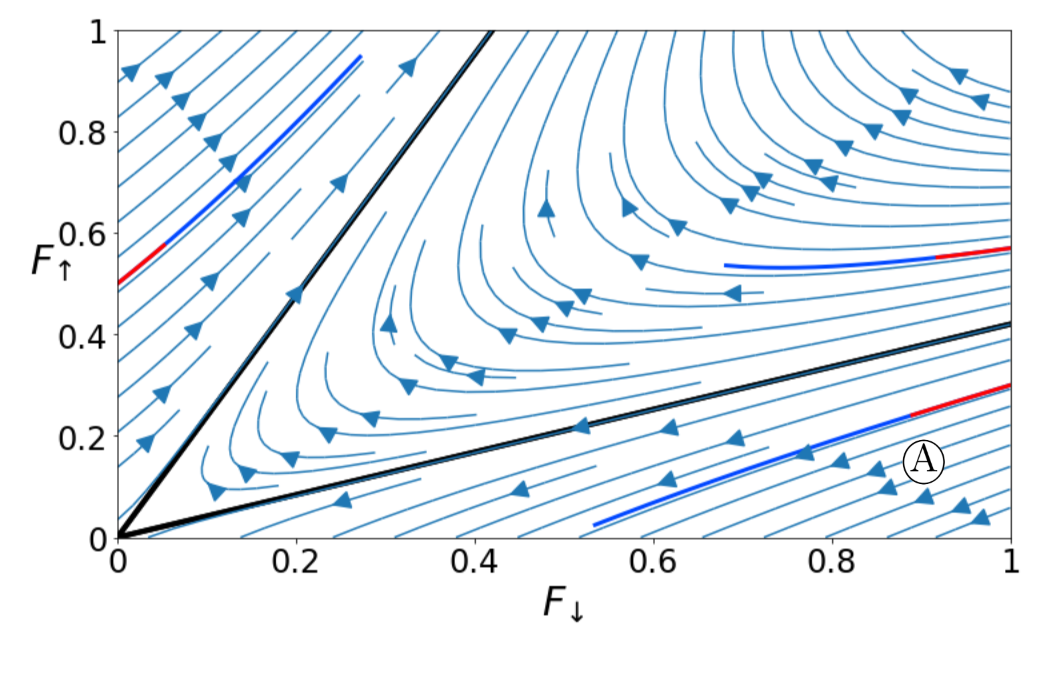
\includegraphics[width=1 \textwidth]{Graphe/bleu_rouge.png}
        \caption{}
        \label{subfig:graph.bleu_rouge}
    \end{subfigure}
    \begin{subfigure}{0.325\textwidth}
        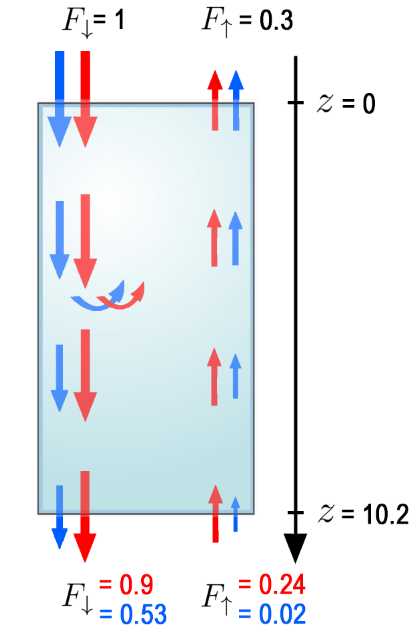
\includegraphics[width=1 \textwidth]{Schema/bleu_rouge.png}
        \caption{}
        \label{subfig:schéma.bleu_rouge}
    \end{subfigure}
    \caption{Comportement des faisceaux lumineux dans l'air dans les longueurs d'onde bleus et rouges lorsque $w=0.83$.}
    \label{fig:air}
    \noindent \justifying
    (a) Graphe de $F_{\uparrow}$ en fonction de $F_{\downarrow}$ avec $g=0$ et $w_{rouge}=w_{bleu}$. Nous constatons que $\tau_{bleu}$ est 5 fois supérieur à $\tau_{rouge}$.
    Les vecteurs propres sont confondus et représentés en noir.\\(b) Comportement des faisceaux lumineux pour les courbes rouges et bleues nommées \textcircled{\small A}, la taille des flèches est proportionnelle à l'intensité du flux lumineux.
\end{figure}

%D'après la figure \ref{fig:air}, nous constatons que le flux à 675nm est plus persistant dans un milieu que le bleu , pourtant cela est contre-intuitif sachant que la longueur d'onde bleue possède un coefficient de diffusion 5 fois supérieur à celui du rouge  comme nous le montre la figure \ref{subfig:Rayleigh} (s'inspirant du phénomène de Rayleigh \cite{cours_Rayleigh}).
%C'est en effet dans ce détail que réside la subtilité, en effet le bleu étant bien plus diffusé que le rouge dans toutes les directions, le flux bleu intense qui poursuit sa trajectoire devient à chaque interaction un flux modéré. Tandis que la lumière de longueur d'onde 675nm est faiblement atténué par l'épaisseur optique.





À l'aide de la diffusion de Rayleigh, nous pouvons expliquer un phénomène du quotidien: la couleur du soleil en fonction de l'orientation du soleil.
La couleur du soleil couchant ou levant paraîtra donc plus rouge car les rayons perçus auront parcouru une plus grande distance dans l'atmosphère car le flux bleu sera plus diffusé (fig: \ref{subfig:soleil}).


\section{Étude du transfert radiatif à travers un nuage}
Nous allons étudier dans cette partie le transfert radiatif à travers un nuage à l'aide du portrait de phase du système à 2 faisceaux.
\begin{figure}[H]
    \centering
    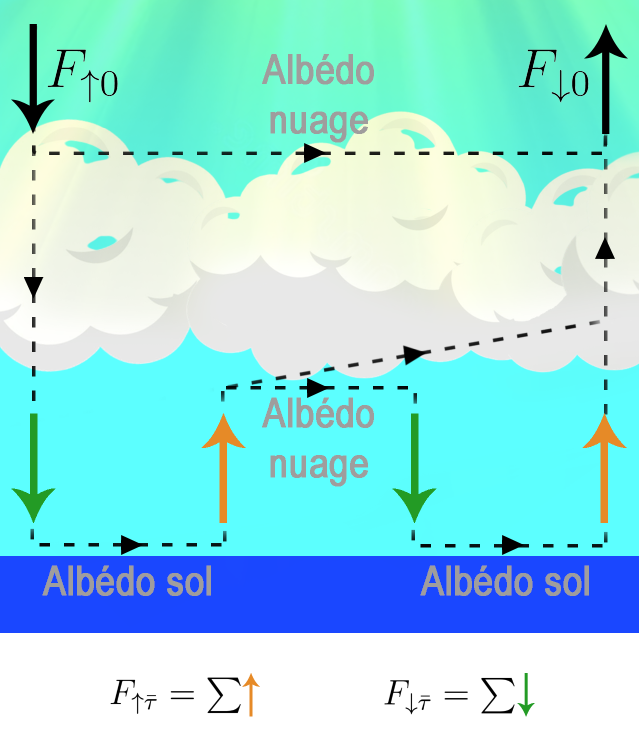
\includegraphics[width=0.5 \textwidth]{Schema/nuage.png}
    \caption{schéma représentant le système complexe: nuage / surface terrestre}
    \label{fig:nuage}
\end{figure}
À l'aide de la figure \ref{fig:nuage} des phénomènes nouveaux sont mis en évidence:
\begin{itemize}
    \item $F_{\downarrow0}$ alimente directement le flux montant $F_{\uparrow0}$ par l'interaction avec la surface du nuage, régie par son albédo.
    \item Le flux descendant $F_{\downarrow\bar{\tau}}$ nourrit le flux montant $F_{\uparrow\bar{\tau}}$ suite à la réflexion sur le sol, ce flux sera donc proportionnel à l'albédo du sol.
    \item Une réflexion en chaîne a lieu entre le sol et le nuage (représenté une seule fois sur la figure) ce qui engendre une somme de flux alimentant $F_{\uparrow0}$.
\end{itemize}
On peut calculer que 
\begin{equation}
    F_{\downarrow\bar{\tau}}=F_{\downarrow\bar{\tau}} + A_{sol}A_{nuage}F_{\downarrow\bar{\tau}} + (A_{sol}A_{nuage})^2F_{\downarrow\bar{\tau}}+\dots+ (A_{sol}A_{nuage})^nF_{\downarrow\bar{\tau}}
\end{equation}
c'est une suite géométrique que l'on peut réécrire à l'aide de la formule de la somme des termes d'une suite géométrique comme
\begin{equation}
    F_{\downarrow\bar{\tau}}=\frac{F_{\downarrow\bar{\tau}}}{1-A_{sol}A_{nuage}}
\end{equation}
car $A_{sol}A_{nuage}<1$ alors quand $n$ tend vers l'infini $(A_{sol}A_{nuage})^n$ tend vers 0. De plus comme $F_{\uparrow\bar{\tau}}$ est obtenu après la réflexion de $F_{\downarrow\bar{\tau}}$ sur le sol:
\begin{equation}
     F_{\uparrow\bar{\tau}}=\frac{A_{sol}F_{\downarrow\bar{\tau}}}{1-A_{sol}A_{nuage}}
\end{equation}
\begin{figure}[H]
    \centering
    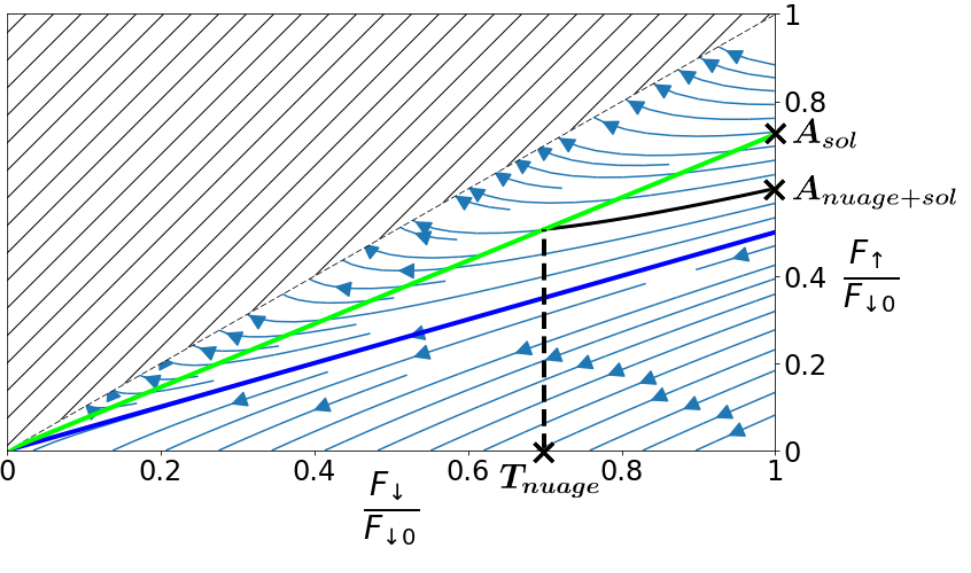
\includegraphics[width=0.7 \textwidth]{Graphe/Albedo Nuage.png}
    \caption{Graphe représentant $\frac{F_{\uparrow}}{F_{\downarrow0}}$ en fonction de $\frac{F_{\downarrow}}{F_{\downarrow0}}$}
    \label{fig:graphnuage}
     \justifying \noindent
    Ce Graphe a été obtenu avec $w=0.9$ et $g=0.2$. La courbe bleue représente le vecteur propre associé à cet espace de phase. La courbe noire correspond à une solution particulière de ce système. La courbe verte est une droite qui fait l'intersection entre l'origine et la fin de la courbe noire.
\end{figure}
Nous pouvons identifier plusieurs, valeurs important sur la figure \ref{fig:graphnuage}. \begin{itemize}
\item L'intersection entre l'axe des ordonnées et de la courbe noire est égale à l'albédo du nuage et du sol, cette valeur est définie comme:
\begin{equation}
    A_{(nuage+sol)}=\frac{F_{\uparrow0}}{F_{\downarrow0}}
\end{equation}
\item La transmittance du nuage $T_{nuage}$ peut se lire l'axe des abscisses au point final de la courbe. La transmittance est définie comme l'intensité lumineuse sortant divisée par celle sortant. Elle est donc définie comme
\begin{equation}
    T_{nuage}=\frac{F_{\downarrow\bar{\tau}}}{F_{\downarrow0}}
\end{equation}
\item La trajectoire du faisceau doit se terminer sur la droite d'équation $\bar{F}_{\uparrow \bar{\tau}}=A_{sol}\bar{F}_{\downarrow \bar{\tau}} $ où $A_{sol}$ est l'abedo du sol.$A_{sol}$ se lit donc sur l'axe des ordonnées. C'est l'intersection de la droite verte avec l'axe des ordonnées.
\end{itemize}
Aucune courbe ne peut se trouver dans la zone hachurée, en effet cela impliquerait que le milieu possède un albédo plus grand que 1, ce qui est physiquement impossible. 

%la courbe verte à une ordonnée supérieure à 1 quand l'abscisse est égale a 1 ce qui implique un albédo supérieur à 1. Cela n’a pas de sens, car ça impliquerait qu’il y a plus de lumière réfléchie que de lumière incidente.

\section{Conclusion}
En conclusion, nous avons pu voir de nombreuses propriétés du modèle à deux faisceaux dans l'espace des phases. Nous avons d'abord vu comment le modèle à deux flux a été établi dans la littérature, puis nous avons calculé les vecteurs et valeurs propres à associer à ce système. À partir de ces valeurs, nous avons pu tracer le portrait de phase des cas simples (simplement avec de la diffusion ou de l'absorption) puis le cas général dans un milieu quelconque. Nous avons ensuite pu démontrer la conservation du volume dans le cas isotrope et que au contraire dans le cas non isotrope, le volume ne se conserve pas. Dans un second temps nous avons déduit les équations du modèle de transfert radiatif aux ordres supérieurs inspiré du modèle à deux faisceaux, avant de nous intéresser aux comportements de différentes longueurs d'onde dans l'eau et dans l'air. Enfin, nous nous sommes intéressés au comportement de la lumière quand un nuage se trouve au-dessus d'un sol réfléchissant.

Nous avons donc une meilleure compréhension des propriétés du portrait de phase dans plusieurs scénarios, mais il en reste plusieurs à explorer. Par exemple l'étude du comportement de la lumière en eau peu profonde où l'on considère que le fond marin (roche, sable, algue) réfléchit la lumière et engendre un flux montant. Cela permettrait d'expliquer les fonds turquoises des eaux caribéennes. Pousser plus loin notre analyse du modèle avec le nuage clarifierait des modèles comme un sol qui réfléchit sélectivement certaines longueurs d'onde comme une prairie, une forêt ou du goudron.

Ce stage a également été une occasion pour nous de découvrir encore plus le monde de la recherche ainsi que de nous familiariser avec les outils de rédaction utilisés en science. En effet, ce rapport a été rédigé sur LaTeX et nous a permis d'avoir une meilleure gestion des figures, des équations et de la numérotation. 

%$\mathbf{T_{nuage}} A_{sol} A_{nuage + sol}$
%\boldsymbol{T_{nuage} A_{sol} A_{nuage + sol}}

%$F_{\uparrow0}$
%$F_{\downarrow0}$
%$F_{\uparrow\bar{\tau}}=\sum$
%$F_{\downarrow\bar{\tau}}=\sum$


\bibliographystyle{IEEEtran} % We choose the "plain" reference style
\bibliography{refs} % Entries are in the refs.bib file
\newpage


\appendix
\section{Bilan Personnel}
Ce stage nous a permis de débloquer de nouvelles compétences, mais également d’en affiner. En effet,
les tâches demandées nous ont obligés à développé et comprendre de nouveaux outils, en l’occurrence en mathématique, physique et informatique avec la découverte dans un premier temps des systèmes dynamiques ainsi que des propriétés matricielles. Dans un second temps, nous avons pu approfondir notre compréhension des interactions entre la lumière et un milieu, et enfin nous avons lu la documentation de fonction informatique que nous avons ensuite détournée pour notre étude.\par
Concernant la documentation, l'exploitation de cours et d'articles on permit d'en affiné notre utilisation et l’extraction d'information.\par
La particularité de ce stage a été l'autonomie ainsi que la pédagogie qu'il a fallu développer. Effectivement, notre maître de stage étant de passage de manière quotidienne nous avons développé une autonomie et une organisation permettant une bonne productivité, de plus notre sujet n'étant pas déjà effectué notre grand enjeu a été de donner des explications claires et de difficulté croissante, d'où la présence de nombreux schéma et graphique, pour le rendre le plus accessible possible.\par
D’un point de vue relationnel, nous avons continué de mieux nous connaître l’un l’autre. En effet, nous avions déjà travaillé ensemble pendant de nombreux mois durant l’APP de L1 et nous avions appris à jouer sur nos forces. Arnaud ayant plus d’aisance avec l’informatique, a rédigé et organisé le programme Python. À l’inverse, Achile étant plus expérimenté avec Photoshop et des logiciels de montage a confectionné les schémas et les ajustements visuels de ce rapport. En revanche, nous débutions tous deux dans l’utilisation de LaTeX, nous avons alors travaillé ensemble pour comprendre le fonctionnement de toutes les commandes, notamment celle des figures et des équations. Lorsque l’on s’approchait d’une impasse, notre superviseur, Cyril DAUPHIN,
venait nous guider tout en nous laissant une grande autonomie pour atteindre nos objectifs. 
\section{Code Python}
Le Code python utiliser pour produire toutes ces figures peut être retrouvé ci-dessous ou sur le lien ici: \url{https://github.com/Danura30082/Code-stage-L2}
\inputminted[baselinestretch=1.2,
fontsize=\footnotesize,
linenos, breaklines]{Python}{V8.py}

\end{document}


